\documentclass{article}
\usepackage{blindtext}
\usepackage{multicol}
\usepackage{amsmath}
\usepackage[spanish]{babel}
\usepackage[T1]{fontenc}
\usepackage{float}
\usepackage{geometry}
 \geometry{
 a4paper,
 total={170mm,257mm},
 left=20mm,
 top=20mm,
 }
\renewcommand{\refname}{Referencias}
\renewcommand{\tablename}{Tabla}
\title{Informe}
\author{Mariona Puente Quera}
\date{2024-07-23}

\usepackage{Sweave}
\begin{document}
\maketitle
\input{Código_informe-concordance}
\section*{Primeros pasos}
\begin{Schunk}
\begin{Sinput}
> if(!require(tinytex)){
+   install.packages('tinytex')
+   library(tinytex)
+ }
\end{Sinput}
\end{Schunk}

\begin{Schunk}
\begin{Sinput}
> tinytex::tlmgr_install('blindtext')
> tinytex::tlmgr_install('amsmath')
> tinytex::tlmgr_install("babel-spanish")
> tinytex::tlmgr_install("grfext")
> tinytex::tlmgr_install("float")
\end{Sinput}
\end{Schunk}

\section*{Objetivos iniciales}
Los objetivos propuestos inicialmente en el proyecto son los siguientes:

\begin{itemize}
    \item \textbf{OBJETIVO GENERAL:} Estudiar cómo correlacionan el apego emocional al propio país y el apego emocional a Europa, y el efecto del género, de la edad y de la nacionalidad en dicha correlación.
    \item \textbf{OBJETIVOS ESPECÍFICOS:}
    \begin{enumerate}
        \item Estudiar y visualizar cómo correlacionan el apego emocional al propio país y el apego emocional a Europa en nuestra muestra.
        \item Estudiar y visualizar los efectos de la variable género en dicha correlación.
        \item Estudiar y visualizar los efectos de la variable edad en dicha correlación.
        \item Estudiar y visualizar los efectos de la variable nacionalidad en dicha correlación.
        \item Estudiar y visualizar cómo correlacionan el apego emocional al propio país y el apego emocional a Europa entre diferentes subgrupos a escoger de entre los diferentes niveles de nuestras variables demográficas.
    \end{enumerate}
\end{itemize}
Con tal de analizar los resultados proporcionados por el dashboard estudiaremos cada objetivo específico por separado a continuación.

\section*{Resultados:}

\section{Estudiar y visualizar cómo correlacionan el apego emocional al propio país y el apego emocional a Europa en nuestra muestra.}

\begin{Schunk}
\begin{Sinput}
> library(ggplot2)
> library(dplyr)
> data <- read.csv('Base de datos depurada.csv')
> df_prop_x <- data %>%
+   filter(!is.na(Apego.emocional.al.propio.país)) %>%
+   group_by(Apego.emocional.al.propio.país) %>%
+   summarise(count = n()) %>%
+   mutate(prop = (count / sum(count)) * 20)
> df_prop_y <- data %>%
+   filter(!is.na(Apego.emocional.a.Europa)) %>%
+   group_by(Apego.emocional.a.Europa) %>%
+   summarise(count = n()) %>%
+   mutate(prop = (count / sum(count)) * 20)
> heatmap_plot <- ggplot(data, aes(x = Apego.emocional.al.propio.país, y = Apego.emocional.a.Europa)) +
+   geom_bin2d(bins = 20, aes(fill = ..count..)) +
+   scale_fill_distiller(palette = "Spectral") +
+   labs(x = "Apego emocional al propio país", y = "Apego emocional a Europa", title = "Mapa de calor") +
+   theme_minimal()
> heatmap_plot <- heatmap_plot +
+   geom_line(data = df_prop_x, aes(x = Apego.emocional.al.propio.país, y = prop), color = "black", size = 1)
> heatmap_plot <- heatmap_plot +
+   geom_path(data = df_prop_y, aes(x = prop, y = Apego.emocional.a.Europa), color = "black", size = 1)
> print(heatmap_plot)
\end{Sinput}
\end{Schunk}
\includegraphics{Código_informe-003}

\section{Estudiar los efectos de la variable género en dicha correlación.}
 \begin{itemize}
 \item D.E. = Desviación estándard
 \item AEPP = Apego emocional al propio país
 \item AEE = Apego emocional a Europa
 \end{itemize}
 \begin{table}[h!]
 \caption{Variable género}
 \begin{tabular}{l | c c c c c}
 \hline
 \bf{Género} & \bf{Media 'AEPP'} & \bf{D.E. 'AEPP'} & \bf{Media 'AEE'} & \bf{D.E. 'AEE'} & \bf{CORR. PEARSON} \\
 \hline
 Mujeres & 7.837861 & 2.145087 & 6.270493 & 2.471481 & 0.4100358 \\
 Hombres & 7.693225 & 2.21015 & 6.097755 & 2.525251 & 0.4146855 \\
 Tod@s & 7.770864 & 2.176612 & 6.190264 & 2.498028 & 0.4128778 \\
 \hline
 \end{tabular}
 \end{table}

 \begin{figure}[H]
 \centering
 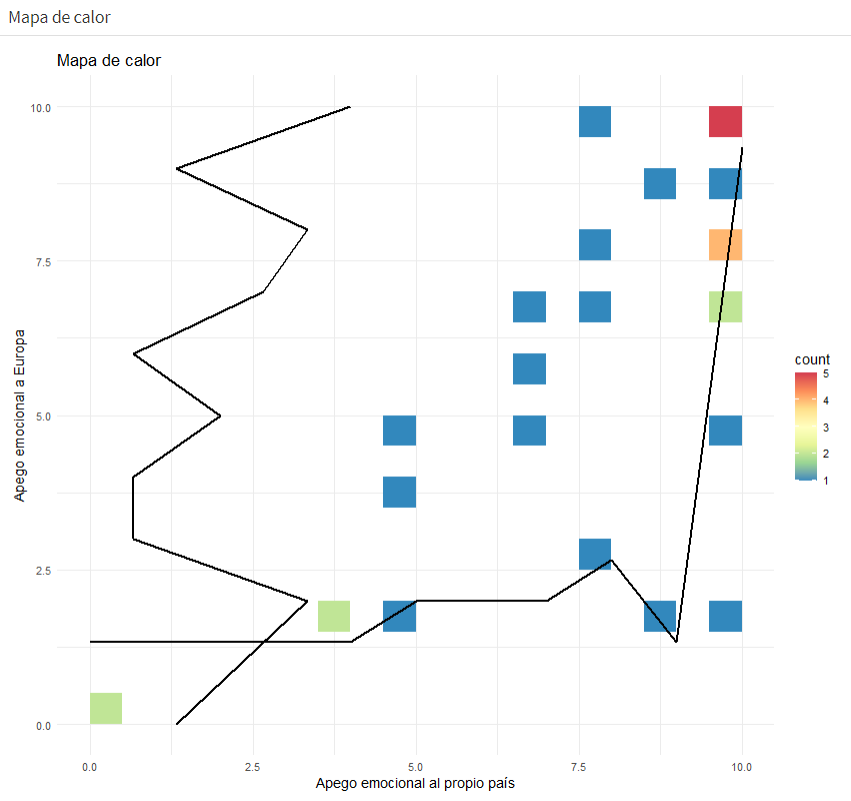
\includegraphics[width=1\textwidth]{Imatge1.png}
 \caption{Visualización de las correlaciones}
 \end{figure}

\section{Estudiar los efectos de la variable edad en dicha correlación.}
 \begin{itemize}
 \item D.E. = Desviación estándard
 \item AEPP = Apego emocional al propio país
 \item AEE = Apego emocional a Europa
 \end{itemize}
 \begin{table}[h!]
 \caption{Variable edad}
 \begin{tabular}{l | c c c c c}
 \hline
 \bf{Rango edad} & \bf{Media 'AEPP'} & \bf{D.E. 'AEPP'} & \bf{Media 'AEE'} & \bf{D.E. 'AEE'} & \bf{CORR. PEARSON} \\
 \hline
 Menores de 30 & 6.926075 & 2.360681 & 6.121974 & 2.354955 & 0.4800369 \\
 Entre 30 y 44 & 7.462656 & 2.19397 & 6.107612 & 2.466652 & 0.4444008 \\
 Entre 45 y 59 & 7.806323 & 2.102556 & 6.191416 & 2.490652 & 0.395468 \\
 Entre 60 y 74 & 8.161118 & 2.020955 & 6.27193 & 2.535688 & 0.3987813 \\
 75 o mayores & 8.466388 & 1.950735 & 6.222835 & 2.643745 & 0.3832552 \\
 Tod@s & 7.770864 & 2.176612 & 6.190264 & 2.498028 & 0.4128778 \\
 \hline
 \end{tabular}
 \end{table}
 
 \begin{figure}[H]
 \centering
 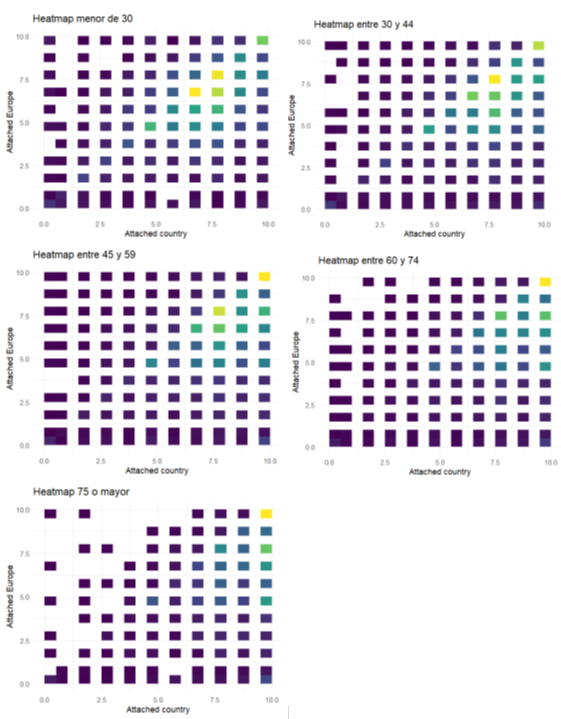
\includegraphics[width=1\textwidth]{Imatge2.png}
 \caption{Visualización de las correlaciones}
 \end{figure}

\section{Estudiar los efectos de la variable nacionalidad en dicha correlación.}
 \begin{itemize}
 \item D.E. = Desviación estándard
 \item AEPP = Apego emocional al propio país
 \item AEE = Apego emocional a Europa
 \end{itemize}
 \begin{table}[h!]
 \caption{Variable nacionalidad}
 \begin{tabular}{l | c c c c c}
 \hline
 \bf{País} & \bf{Media 'AEPP'} & \bf{D.E. 'AEPP'} & \bf{Media 'AEE'} & \bf{D.E. 'AEE'} & \bf{CORR. PEARSON} \\
 \hline
 Alemania & 7.212096 & 2.234437 & 6.486509 & 2.356144 & 0.5506882 \\
 Áustria & 8.36 & 1.829636 & 6.524541 & 2.3696 & 0.2826011 \\
 Croacia & 7.798714 & 2.247549 & 5.990909 & 2.59227 & 0.4341063 \\
 Eslovaquia & 7.570231 & 2.426643 & 5.966878 & 2.792222 & 0.4622578 \\
 Eslovenia & 7.753017 & 2.212389 & 5.930138 & 2.597684 & 0.458533 \\
 Finlandia & 8.630198 & 1.56143 & 6.838132 & 1.964155 & 0.3117515 \\
 Hungría & 8.167143 & 2.017117 & 7.1415 & 2.386804 & 0.4656425 \\
 Irlanda & 7.968688 & 1.918663 & 5.943641 & 2.399126 & 0.3305107 \\
 Lituania & 7.807777 & 2.296271 & 5.890895 & 2.731617 & 0.2824732 \\
 Noruega & 8.405101 & 1.668298 & 6.596847 & 2.154182 & 0.3667099 \\
 Países Bajos & 6.894737 & 2.092995 & 5.722584 & 2.187825 & 0.4928814 \\
 Reino Unido & 6.575758 & 2.731243 & 4.795679 & 2.788772 & 0.2884089 \\
 Suiza & 7.926705 & 1.826457 & 6.066909 & 2.297686 & 0.297761 \\
 Tod@s & 7.770864 & 2.176612 & 6.190264 & 2.498028 & 0.4128778 \\
 \hline
 \end{tabular}
 \end{table}

 \begin{figure}[H]
 \centering
 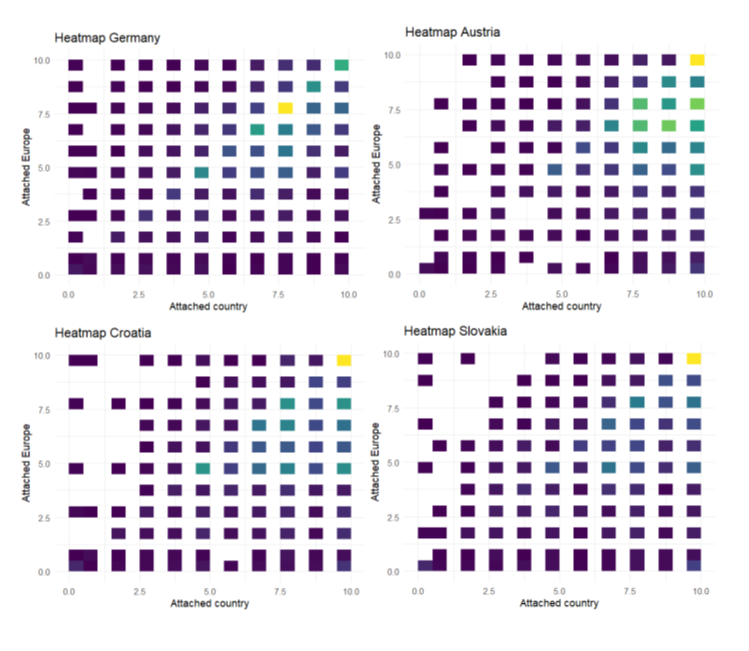
\includegraphics[width=1\textwidth]{Imatge3.png}
 \caption{Visualización de las correlaciones}
 \end{figure}

 \begin{figure}[H]
 \centering
 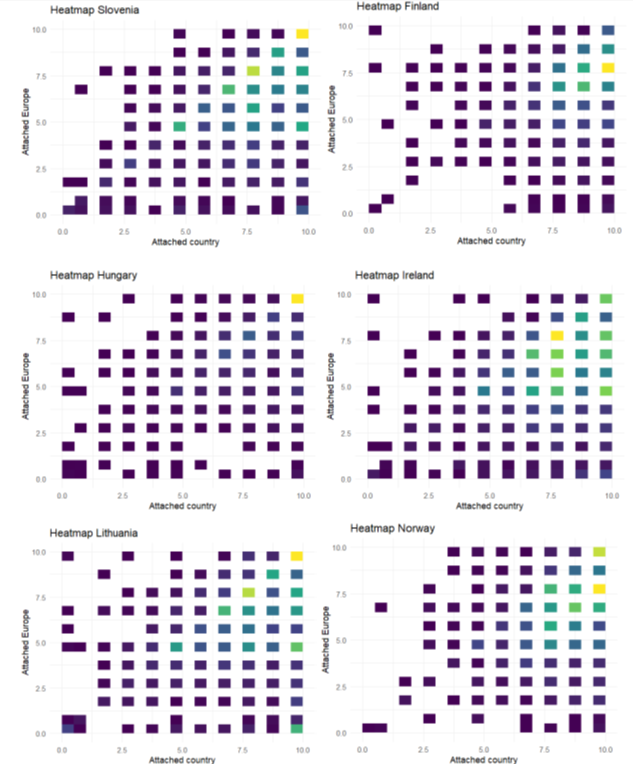
\includegraphics[width=1\textwidth]{Imatge4.png}
 \caption{}
 \end{figure}

 \begin{figure}[H]
 \centering
 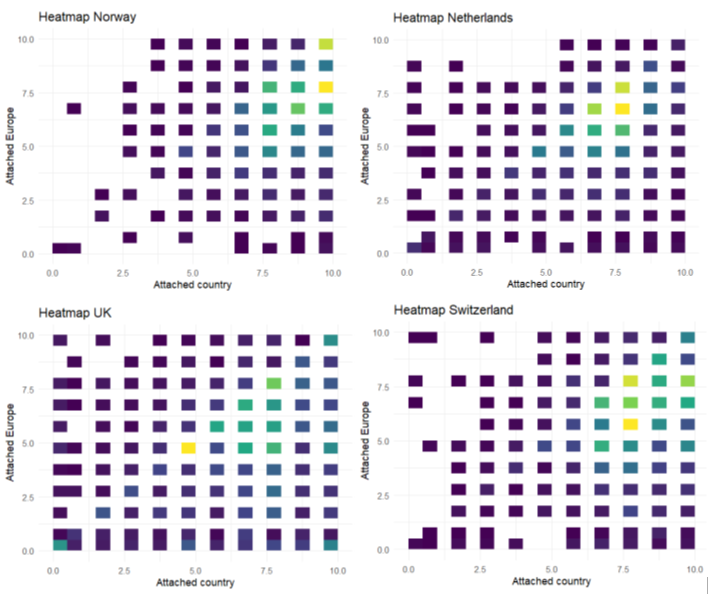
\includegraphics[width=1\textwidth]{Imatge5.png}
 \caption{Visualización de las correlaciones}
 \end{figure}

\section{Estudiar cómo correlacionan el apego emocional al propio país y el apego emocional a Europa entre diferentes subgrupos a escoger de entre los diferentes niveles de nuestras variables demográficas.}

\section*{Conclusiones}

Lógicamente la última fila de cada tabla es la misma, puesto que está compuesta de la muestra completa.

\end{document}
